\section{Exemplos de Máquinas de Turing}

\begin{frame}[fragile]{Exemplo: Duplicando o número de traços}

    Assuma que a máquina abaixo começa no traço mais à esquerda de um bloco de $n$ traços de uma 
    fita que, de resto, está em branco. Esta máquina para no traço mais à esquerda de um bloco de
    $2n$ traços de uma fita que, de resto, está em branco.
    \begin{figure}[h]
        \centering
        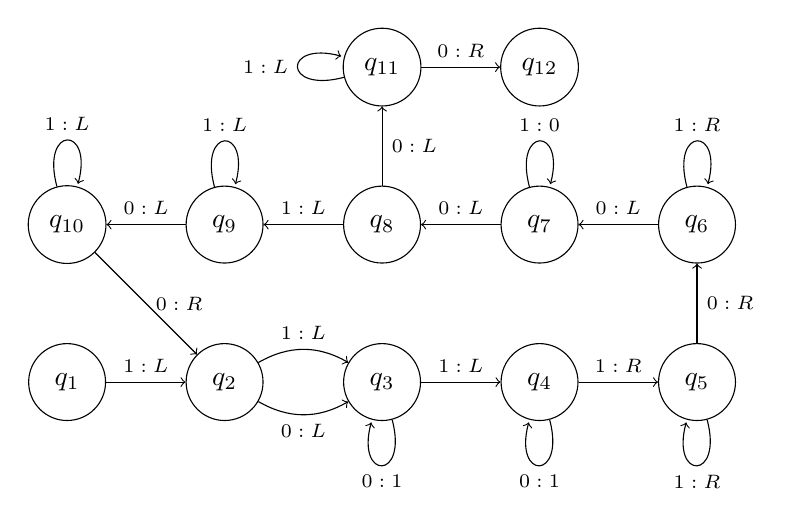
\begin{tikzpicture} 
            \node[draw,circle,minimum size=8pt,inner sep=6pt] (q1) at (0, 0) { $q_1$ };
            \node[draw,circle,minimum size=8pt,inner sep=6pt] (q2) at (2, 0) { $q_2$ };
            \node[draw,circle,minimum size=8pt,inner sep=6pt] (q3) at (4, 0) { $q_3$ };
            \node[draw,circle,minimum size=8pt,inner sep=6pt] (q4) at (6, 0) { $q_4$ };
            \node[draw,circle,minimum size=8pt,inner sep=6pt] (q5) at (8, 0) { $q_5$ };
            \node[draw,circle,minimum size=8pt,inner sep=6pt] (q6) at (8, 2) { $q_6$ };
            \node[draw,circle,minimum size=8pt,inner sep=6pt] (q7) at (6, 2) { $q_7$ };
            \node[draw,circle,minimum size=8pt,inner sep=6pt] (q8) at (4, 2) { $q_8$ };
            \node[draw,circle,minimum size=8pt,inner sep=6pt] (q9) at (2, 2) { $q_9$ };
            \node[draw,circle,minimum size=8pt,inner sep=5pt] (q10) at (0, 2) { $q_{10}$ };
            \node[draw,circle,minimum size=8pt,inner sep=5pt] (q11) at (4, 4) { $q_{11}$ };
            \node[draw,circle,minimum size=8pt,inner sep=5pt] (q12) at (6, 4) { $q_{12}$ };

            \draw[->] (q1) edge node[anchor=south] { \scriptsize $1:L$ } (q2);
            \draw[->] (q2) edge[bend left] node[anchor=south] { \scriptsize $1:L$ } (q3);
            \draw[->] (q2) edge[bend right] node[anchor=north] { \scriptsize $0:L$ } (q3);
            \draw[->] (q3) edge node[anchor=south] { \scriptsize $1:L$ } (q4);
            \draw[->] (q3) edge[loop below]  node { \scriptsize $0:1$ } (q4);
            \draw[->] (q4) edge node[anchor=south] { \scriptsize $1:R$ } (q5);
            \draw[->] (q4) edge[loop below]  node { \scriptsize $0:1$ } (q4);
            \draw[->] (q5) edge node[anchor=west] { \scriptsize $0:R$ } (q6);
            \draw[->] (q5) edge[loop below]  node { \scriptsize $1:R$ } (q5);
            \draw[->] (q6) edge node[anchor=south] { \scriptsize $0:L$ } (q7);
            \draw[->] (q6) edge[loop above]  node { \scriptsize $1:R$ } (q6);
            \draw[->] (q7) edge node[anchor=south] { \scriptsize $0:L$ } (q8);
            \draw[->] (q7) edge[loop above]  node { \scriptsize $1:0$ } (q7);
            \draw[->] (q8) edge node[anchor=south] { \scriptsize $1:L$ } (q9);
            \draw[->] (q9) edge node[anchor=south] { \scriptsize $0:L$ } (q10);
            \draw[->] (q9) edge[loop above]  node { \scriptsize $1:L$ } (q9);
            \draw[->] (q10) edge node[anchor=west] { \scriptsize $0:R$ } (q2);
            \draw[->] (q10) edge[loop above]  node { \scriptsize $1:L$ } (q10);
            \draw[->] (q8) edge node[anchor=west] { \scriptsize $0:L$ } (q11);
            \draw[->] (q11) edge node[anchor=south] { \scriptsize $0:R$ } (q12);
            \draw[->] (q11) edge[loop left]  node { \scriptsize $1:L$ } (q11);

        \end{tikzpicture} 
    \end{figure}

\end{frame}

\begin{frame}[fragile]{Configurações para uma máquina com $n = 2$}

    \begin{itemize}
        \item A configuração inicial da máquina é
        \[
            1_11
        \]

        \item O estado $1$ move o computador para à esquerda, levando à configuração
        \[
            0_211
        \]

        \item Como o computador está avaliando um quadrado vazio, as próximas configurações
            são
        \[
            0_3011,\ \ 1_3011,\ \ 0_41011,\ \ 1_41011
        \]
        \item Esta sequência de instruções criou um par de traços à esquerda do bloco original,
            separado deste por um espaço em branco
    \end{itemize}

\end{frame}

\begin{frame}[fragile]{Configurações para uma máquina com $n = 2$}

    \begin{itemize}
        \item Os dois próximos estados ($5$ e $6$) movimentam o computador para o último traço
            do segundo bloco (bloco original):
        \[
            11_5011,\ \ 110_511,\ \ 1101_61,\ \ 11011_6,\ \ 110110_6,\ \ 11011_7
        \]

        \item O estado $7$ apaga o último traço do bloco (se existir), e em seguida segue para
            à esquerda
        \[
            11010_7,\ \ 1101_8
        \]

        \item Como há ainda um traço no bloco original, o estado $8$ segue para o $9$, que
            salta o bloco original, e em seguida para o $10$, que posiciona a máquina no último
            traço do bloco à esquerda:
        \[
            110_91,\ \ 11_{10}01,\ \ 1_{10}101,\ \ 0_{10}1101
        \]
    \end{itemize}

\end{frame}

\begin{frame}[fragile]{Configurações para uma máquina com $n = 2$}

    \begin{itemize}
        \item De volta ao estado $2$, a máquina segue para escrever mais um par de traços à 
            esquerda do bloco à esquerda:
        \[
            1_2101,\ \ 0_31101,\ \ 1_31101,\ \ 0_411101,\ \ 1_411101
        \]

        \item Novamente os estados $5$ e $6$ posicionarão o computador no último traço do bloco
            original:
        \[
            11_51101,\ \ 111_5101,\ \ 1111_501,\ \ 11110_51, \ \ 111101_6, \ \ 1111010_6
        \]

        \item O estado $7$ apaga o último traço restante, e segue para o estado $8$:
        \[
            111101_7, \ \ 111100_7, \ \ 11110_8
        \]

        \item Como não há mais traços no bloco original, o estado $8$ vai para o estado $11$, o
            qual irá posicionar o computador no traço mais à esquerda do bloco restante:
        \[
            1111_{11},\ \ 111_{11}1,\ \ 11_{11}11,\ \ 1_{11}111,\ \ 0_{11}1111,\ \ 1_{12}111
        \]
    \end{itemize}

\end{frame}

\begin{frame}[fragile]{Exemplo: Paridade}

    A máquina abaixo inicia no traço mais à esquerda de um bloco de $n$ traços de uma fita que,
    de resto, está em branco, e termina em um quadrado de uma fita, que de resto está em branco,        que contém um traço, se $n$ é ímpar, ou está em branco, se $n$ é par.

    \vspace{0.3in}
    
    \begin{figure}[h]
        \centering
        \begin{tikzpicture}[opacity=0]
            \node[draw,circle] (q1) at (0, 0) { $\mathbf{1}$ };
            \node[draw,circle] (q2) at (3, 2) { $\mathbf{2}$ };
            \node[draw,circle] (q3) at (6, 0) { $\mathbf{3}$ };
            \node[draw,circle] (q4) at (3, -2) { $\mathbf{4}$ };
            \node[draw,circle] (q5) at (9, 0) { $\mathbf{5}$ };

            \draw[->] (q1) edge node[anchor=south east] { \footnotesize $1:B$ } (q2);
            \draw[->] (q2) edge node[anchor=south west] { \footnotesize $B:R$ } (q3);
            \draw[->] (q3) edge node[anchor=north west] { \footnotesize $1:B$ } (q4);
            \draw[->] (q3) edge node[anchor=south] { \footnotesize $B:1$ } (q5);
            \draw[->] (q4) edge node[anchor=north east] { \footnotesize $B:R$ } (q1);
        \end{tikzpicture}
    \end{figure}

\end{frame}

\begin{frame}[fragile]{Exemplo: Paridade}

    A máquina abaixo inicia no traço mais à esquerda de um bloco de $n$ traços de uma fita que,
    de resto, está em branco, e termina em um quadrado de uma fita, que de resto está em branco,        que contém um traço, se $n$ é ímpar, ou está em branco, se $n$ é par.

    \vspace{0.3in}
    
    \begin{figure}[h]
        \centering
        \begin{tikzpicture}[opacity=1]
            \node[draw,circle] (q1) at (0, 0) { $\mathbf{1}$ };
            \node[draw,circle] (q2) at (3, 2) { $\mathbf{2}$ };
            \node[draw,circle] (q3) at (6, 0) { $\mathbf{3}$ };
            \node[draw,circle] (q4) at (3, -2) { $\mathbf{4}$ };
            \node[draw,circle] (q5) at (9, 0) { $\mathbf{5}$ };

            \draw[->] (q1) edge node[anchor=south east] { \footnotesize $1:B$ } (q2);
            \draw[->] (q2) edge node[anchor=south west] { \footnotesize $B:R$ } (q3);
            \draw[->] (q3) edge node[anchor=north west] { \footnotesize $1:B$ } (q4);
            \draw[->] (q3) edge node[anchor=south] { \footnotesize $B:1$ } (q5);
            \draw[->] (q4) edge node[anchor=north east] { \footnotesize $B:R$ } (q1);
        \end{tikzpicture}
    \end{figure}

\end{frame}


\begin{frame}[fragile]{Configurações em uma máquina com $n=3$}

    \begin{itemize}
        \item A configuração inicial da máquina é
        \[
            1_111
        \]

        \item Como o quadrado a ser avaliado tem um traço, o computador 
            apaga o traço, seguindo para os estados $2$ e $3$:
        \[
            0_211,\ \ 1_31
        \]

        \item Encontrando um traço no quadrado, o estado $3$ também o apaga, e retorna para o
            estado inicial, passando pelo estado $4$:
        \[
            0_41,\ \ 1_1
        \]

    \end{itemize}

\end{frame}

\begin{frame}[fragile]{Configurações em uma máquina com $n=3$}

    \begin{itemize}
        \item Novamente no estado $1$, o computador torna a apagar o traço, seguindo para o 
            estado $3$:
        \[
            0_2,\ \ 0_3
        \]

        \item Agora o estado $3$ encontra um quadrado em branco (de fato, a fita está toda em
            branco neste momento)

        \item Neste caso, ele escreve um traço no quadrado e vai para estado $5$, onde a 
            computação é encerrada:
        \[
            1_5
        \]

        \item Se $n$ fosse par, a computação se encerraria no estado $1$, em um quadrado em branco
    \end{itemize}

\end{frame}

\begin{frame}[fragile]{Exemplo: Adição de números positivos}

    A máquina abaixo inicia no traço mais à esquerda de um bloco de $n$ traços, o qual é seguido
    de um quadrado com um espaço em branco, e mais um bloco de $m$ traços: de resto, a fita está
    em branco. Ela termina a computação no traço mais à esquerda de um bloco de $m+n$ traços, e 
    o restante da fita está em branco.

    \vspace{0.3in}
    
    \begin{figure}[h]
        \centering
        \begin{tikzpicture}[opacity=0]
            \node[draw,circle] (q1) at (0, 0) { $\mathbf{1}$ };
            \node[draw,circle] (q2) at (2.5, 0) { $\mathbf{2}$ };
            \node[draw,circle] (q3) at (5, 0) { $\mathbf{3}$ };
            \node[draw,circle] (q4) at (7.5, 0) { $\mathbf{4}$ };

            \draw[->] (q1) edge[loop above] node { \footnotesize $1:B$ } (q2);
            \draw[->] (q1) edge node[anchor=south] { \footnotesize $B:R$ } (q2);
            \draw[->] (q2) edge[loop above] node { \footnotesize $1:R$ } (q2);
            \draw[->] (q2) edge node[anchor=south] { \footnotesize $B:1$ } (q3);
            \draw[->] (q3) edge[loop above] node { \footnotesize $1:L$ } (q3);
            \draw[->] (q3) edge node[anchor=south] { \footnotesize $B:R$ } (q4);
        \end{tikzpicture}
    \end{figure}

\end{frame}

\begin{frame}[fragile]{Exemplo: Adição de números positivos}

    A máquina abaixo inicia no traço mais à esquerda de um bloco de $n$ traços, o qual é seguido
    de um quadrado com um espaço em branco, e mais um bloco de $m$ traços: de resto, a fita está
    em branco. Ela termina a computação no traço mais à esquerda de um bloco de $m+n$ traços, e 
    o restante da fita está em branco.

    \vspace{0.3in}
    
    \begin{figure}[h]
        \centering
        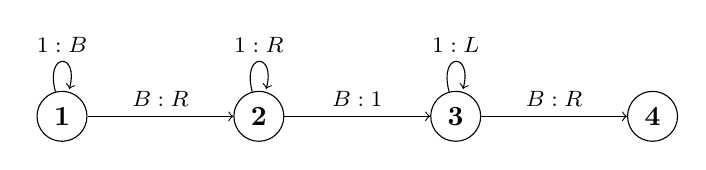
\begin{tikzpicture}[opacity=1]
            \node[draw,circle] (q1) at (0, 0) { $\mathbf{1}$ };
            \node[draw,circle] (q2) at (2.5, 0) { $\mathbf{2}$ };
            \node[draw,circle] (q3) at (5, 0) { $\mathbf{3}$ };
            \node[draw,circle] (q4) at (7.5, 0) { $\mathbf{4}$ };

            \draw[->] (q1) edge[loop above] node { \footnotesize $1:B$ } (q2);
            \draw[->] (q1) edge node[anchor=south] { \footnotesize $B:R$ } (q2);
            \draw[->] (q2) edge[loop above] node { \footnotesize $1:R$ } (q2);
            \draw[->] (q2) edge node[anchor=south] { \footnotesize $B:1$ } (q3);
            \draw[->] (q3) edge[loop above] node { \footnotesize $1:L$ } (q3);
            \draw[->] (q3) edge node[anchor=south] { \footnotesize $B:R$ } (q4);
        \end{tikzpicture}
    \end{figure}

\end{frame}

\begin{frame}[fragile]{Configurações em uma máquina com $n=2, m = 3$}

    \begin{itemize}
        \item A configuração inicial da máquina é
        \[
            1_110111
        \]

        \item O estado $1$ apaga o primeiro traço e segue para o estado $2$:
        \[
            0_110111,\ \ 1_20111
        \]

        \item O estado $2$ localiza o espaço em branco que separa os dois blocos, escreve um traço
            no quadrado correspondente e segue para o estado $3$:
        \[
            10_2111,\ \ 11_3111
        \]

        \item Por fim, o estado $3$ posiciona o computador no traço mais à esquerda do bloco
            recém-formado:
        \[
            1_31111,\ \ 0_311111,\ \ 1_41111
        \]
    \end{itemize}

\end{frame}
%% TODO:
% - Exemplos da máquina de adição
% - Incluir seção sobre computabilidade e tese de Turing
% - Incluir aula sobre incomputabilidade (problema da parada)
